\documentclass[a4, 12pt]{article}
\usepackage[english]{babel}
\usepackage[utf8]{inputenc}
\usepackage{graphicx}
\usepackage{fancyhdr}
\usepackage{float}
\usepackage{graphicx}
\usepackage{subcaption}
\usepackage{caption}
\usepackage{amsmath}
\usepackage{booktabs}
\usepackage{tikz}  
\usetikzlibrary{arrows.meta}
\usepackage{hyperref}
\pagestyle{fancy}
\fancyhf{}
\lhead{Syed babar ali school of science and engineering, LUMS}
\cfoot{\thepage}
%\rfoot{Student Name: Raees}
\renewcommand{\headrulewidth}{0.5pt}
\renewcommand{\footrulewidth}{0.5pt}

\begin{document}

\begin{titlepage}

\begin{figure}
   \begin{minipage}{0.48\textwidth}
   \begin{flushleft}
     
\includegraphics[scale=0.5]{Images/LOGO.png}
   \end{flushleft}
   \end{minipage}\hfill
   %\begin{minipage}{0.48\textwidth}
  % \begin{flushright}
  %   \includegraphics[scale=0.2]{Images/ITU Seal.png}
  % \end{flushright}
  % \end{minipage}
\end{figure}

\thispagestyle{fancy}

\vspace{1in}

\center

\textsc{\large AI651 – Deep Learning for Space, Time and Graphs}

\vspace{0.5in}

\noindent\makebox[\linewidth]{\rule{\linewidth}{1.2pt}}
\textsc{ \textbf{\large Assignment 01 }}
\noindent\makebox[\linewidth]{\rule{\linewidth}{1.2pt}}

\vspace{0.5in}

\begin{minipage}{0.48\textwidth}
    \begin{flushleft}
        %\textit{Student:} \\
        Student Name: Maria Rafique  \\
        Student ID:  25280077 \\
        Semester: Fall 2026\\
      \textbf{Github Code Link:} 
\href{https://github.com/Goat8/Forecasting-Across-Heterogeneous-Sensors.git}{PA1 Forecasting-Across-Heterogeneous-Sensors}

        \vspace{10pt}
    %\end{flushleft}
%\end{minipage}
%\begin{minipage}{0.48\textwidth}
   % \begin{flushright}
    %\textit{Supervisor:} \\
    % Supervisor Name: Dr. Moshin Ali\\ 
    \vspace{14pt}
    %Signature:$-------$
    %\end{flushright}
    \end{flushleft}
\end{minipage}

\vspace{2in}

\textbf{\large Syed babar ali school of science and engineering, LUMS} \\
  \vspace{14pt}

\today

\end{titlepage}

\newpage
\setcounter{page}{2}
\tableofcontents
\newpage

\section{ Task 1 Forecasting across heterogenous sensors}
\subsection{Response 1A. Predict, measure, and revise the aggregate ordering.}
\paragraph{Prediction before Output 1.1}
Before running experiment my expected ordering is follows:
\paragraph{Station 1 ,2 ,3}

\begin{table}[htbp]
\centering
\caption{Expected Performance Ranking for Established Stations}
\label{tab:established_ranking}
\vspace{2mm}
\begin{tabular}{@{} l c c c c @{}}
\toprule
\textbf{Rank Order} & \textbf{1st (Best)} & \textbf{2nd} & \textbf{3rd} & \textbf{4th} \\
\midrule
\textbf{Model Name} & Raw Attention & Period-routed Ridge & Sensor-specific Ridge & Shared Ridge \\
\bottomrule
\end{tabular}
\end{table}

because raw attention can achieve the strongest forecasting performance due to its architectural flexibility as it look for temporal mixing based on the current context unlike fixed mapping approaches. so, attention has enough flexibility to learn context-dependent temporal relationships.
Period-routed Ridge can rank second because it has to be provided with an explicit information designed to incorporate operating periods, which causes strong adaptability even though it lacks full context flexibility. 
Sensor-specific Ridge can outperforms Shared Ridge by utilizing customized station-tailored parameter mappings and in last Shared Ridge because it relies on a single fixed mapping applied across all stations.

\paragraph{Held-out Station 4}

\begin{table}[htbp]
\centering
\caption{Expected Performance Ranking for Held-out Station 4}
\label{tab:heldout_ranking}
\vspace{2mm}
\begin{tabular}{@{} l c c c c @{}}
\toprule
\textbf{Rank Order} & \textbf{1st (Best)} & \textbf{2nd} & \textbf{3rd} & \textbf{Unevaluated} \\
\midrule
\textbf{Model Name} & Raw Attention & Period-routed Ridge & Shared Ridge & Sensor-specific Ridge* \\
\bottomrule
\end{tabular}
\\[1.5ex]
\raggedright \footnotesize{*Sensor-specific Ridge cannot be evaluated on Station 4.}
\end{table}

For the held-out Station 4, Raw Attention performs would still do best because it can adapt its temporal mixing based on the available context. Period-routed Ridge would come next, as it adjust its predictions according to the estimated vibration period (operating pace). Shared Ridge ranks third and serves as a more general baseline with fixed mappings. Sensor-specific Ridge cannot be used here because it needs parameters trained specifically for each station, and Station 4 was not included during training.

\paragraph{Actual  Output 1.1}
Based on RMSE the ranking turned out different. 

\begin{table}[htbp]
\centering
\caption{Observed Performance Ranking (RMSE, m/s$^2$) for Established Stations and Held-out Station 4}
\label{tab:observed_ranking}
\vspace{2mm}
\resizebox{\textwidth}{!}{%
\begin{tabular}{@{} l c c c c @{}}
\toprule
\textbf{Station Group} & \textbf{1st (Best)} & \textbf{2nd} & \textbf{3rd} & \textbf{4th} \\
\midrule
\textbf{Established (1, 2, 3)} &
  \shortstack{Period-routed Ridge \\ 0.166} &
  \shortstack{Raw Attention \\ 0.434} &
  \shortstack{Shared Ridge \\ 0.767} &
  \shortstack{Sensor-specific Ridge \\ 0.768} \\
\addlinespace
\textbf{Held-out Station 4} &
  \shortstack{Period-routed Ridge \\ 0.173} &
  \shortstack{Raw Attention \\ 0.665} &
  \shortstack{Shared Ridge \\ 0.876} &
  \shortstack{Sensor-specific Ridge* \\ unavailable} \\
\bottomrule
\end{tabular}%
}
\\[1.5ex]
\raggedright \footnotesize{*Sensor-specific Ridge cannot be evaluated on Station 4 because it has no parameters trained for that station.}
\end{table}

\paragraph{Established stations.}
Period-routed Ridge performed best across all three products, with RMSE values ranging from \(0.152\) to \(0.181\). Its overall RMSE is \(0.166\), compared to \(0.434\) for Raw Attention and \(0.767\) for Shared Ridge. This means its RMSE is about \(2.6\times\) lower than Raw Attention and \(4.6\times\) lower than Shared Ridge.

Raw Attention ranked second. Its RMSE was about \(43\%\) lower than that of Shared Ridge, although it still performed worse than Period-routed Ridge.

Shared Ridge and Sensor-specific Ridge performed very similarly across all three products. Their RMSE differences were at most \(0.009\). This shows that using a separate linear mapping for each station provides little benefit in this experiment despite increasing the number of parameters from \(4{,}608\) to \(13{,}824\).

\paragraph{Held-out Station 4.}
The ordering remained unchanged but the gaps between the models became larger so trend is similar.
Period-routed Ridge changed only slightly, from \(0.166\) to \(0.173\) RMSE, which is an increase of about \(4\%\). 
Shared Ridge increases from \(0.767\) to \(0.876\),  increased of about \(14\%\). 
Raw Attention showed the largest increase from \(0.434\) to \(0.665\), or about \(53\%\).
The advantage of Period-routed Ridge over Raw Attention therefore increased from about \(2.6\times\) on the established stations to \(3.8\times\) on Station 4. 
Raw Attention still performs better than Shared Ridge on the held-out station, but the difference is smaller: its RMSE was about \(24\%\) lower than Shared Ridge.
Sensor-specific Ridge couldnot be evaluated on Station 4 because the station was completely held out from fitting, so no station-specific parameters were learned for it.

\paragraph{Across products.}
The product-wise results showed different levels of sensitivity to the operating regime. 
For Shared Ridge Product B has the highest RMSE (\(0.854\)), while Product C has the lowest (\(0.621\)). 
Sensor-specific Ridge showed a similar pattern with RMSE values of \(0.804\), \(0.852\), and \(0.630\) for Products A, B, and C, respectively.
Raw Attention has a smaller variation across products. Its RMSE giving spread of about \(0.06\) only. 
And Period-routed Ridge had the smallest spread of about \(0.02\) only across products
This showed that the global ridge models are more sensitive to the operating product while Raw Attention and  Period-routed Ridge maintained more consistent error across products. 
This is consistent with Period-routed Ridge as its using the estimated period to choose the relevant forecasting rule..

\begin{table}[htbp]
\centering
\caption{}
\label{tab:model_performance}
\resizebox{\linewidth}{!}{%
\begin{tabular}{lcccc}
\toprule
\textbf{Model} & \textbf{Product A RMSE} & \textbf{Product B RMSE} & \textbf{Product C RMSE} & \textbf{Spread ($\max - \min$)} \\
\midrule
Shared Ridge          & 0.805 & 0.854 & 0.621 & 0.233 \\
Sensor-specific Ridge & 0.804 & 0.852 & 0.630 & 0.222 \\
Period-routed Ridge   & 0.181 & 0.164 & 0.152 & 0.029 \\
Raw Attention         & 0.428 & 0.467 & 0.403 & 0.064 \\
\bottomrule
\end{tabular}%
}
\end{table}
\paragraph{Revised Expected Ordering}
My prediction was wrong in two places.
\begin{itemize}
  \item \textbf{Raw Attention and Period-routed Ridge swapped places} on both station
  populations. I expected the flexibility of attention would outweigh the hand-designed
  period information but opposite happened and the margin is large (2.6--3.8$\times$).
  \item \textbf{Sensor-specific Ridge did not beat Shared Ridge.} The two are tied
  (0.768 vs.\ 0.767), so the 3rd/4th ranking on the established stations its not real difference..
\end{itemize}
The prediction that Shared Ridge is third on Station 4 was correct. The revised
ordering is therefore: \textbf{Period-routed Ridge $>$ Raw Attention $>$ Shared Ridge
$\approx$ Sensor-specific Ridge} on the established stations, and
\textbf{Period-routed Ridge $>$ Raw Attention $>$ Shared Ridge} on Station 4.

\paragraph{Differences through model asssumptions}

\paragraph{Shared Ridge.}
It assumes that one linear forecasting rule is suitable for all stations and all products. But the vibration period changes with the product. 
For example Product A has a period of about \(16\) samples, while Product C has a period of about \(30\) samples. The same fixed linear rule therefore has to handle different repeating patterns. 
It cannot adapt its forecasting rule when the period changes so it learns a compromise that works poorly across the different regimes. This also explains its relatively high RMSE. the model does not show a very large increase in error on the held-out station pointing that its main problem is the fixed forecasting rule rather than station-specific overfitting.

\paragraph{Sensor-specific Ridge.} It assumes that the main source of variation
is the \emph{station}. but results showed that this assumption is wrong: giving each
station its own mapping changed the RMSE by at most 0.009 on any product. The
variation that matters is between \emph{products and periods} and each station still
saw a mixture of periods so each per-station map faces the same compromise as the
shared model. Also it cannot be applied to a station it has not seen yet.

\paragraph{Period-routed Ridge.} It assumes that the dynamics are determined by
the period of the signal and that once the period is known a linear mapping is
sufficient. This matched the structure of the data: splitting by period removed the
compromise that hurt the global models which explains the 4.6$\times$ improvement
over Shared Ridge and the nearly flat error across products (0.152--0.184). Because
the period is a property of the signal itself rather than of the station, the
routing transfers directly to Station 4, giving the smallest generalisation gap (+4\%).
Its only noticeable degradation is on Product B at Station 4 (+11\%). A clear
explanation is that Station 4's Product B period is represented less well by the
trained routes, but this would need to be checked.

\paragraph{Raw Attention.} It makes the fewest assumptions: so it must discover any
periodic structure from data using learned position embeddings, content-based
mixing and a flattened linear head. Its flexibility let it capture some of the
periodic structure which explains the 43\% improvement over Shared Ridge. However, it
has 368k parameters and about 80\% of which sit in the forecast head that maps each
absolute position directly to the output, and it is trained for only 6{,}000 steps.
It therefore partly fits patterns specific to the training stations, which explained
the 53\% drop on Station 4. 

\paragraph{Conclusion.} The ranking followed how well each model's assumptions match
the data rather than how flexible the model is. The dominant structure is
period-dependent approximately linear dynamics. The model that encoded this
explicitly is the most accurate and the most stable across products and stations, and
among the cheapest. The fully flexible model is second but failed to discover this
structure reliably. The models that assume a single mapping, or a per-station mapping,
cannot represent it at all.
Why station identity isn't enough?
There are four stations but the same station can experience Product A → Product B → Product C → so Station 1 doesn't always need the same forecasting rule.
\textbf{Its current operating context matters more.} How much does the right inductive bias matter compared with a more flexible model?


\subsubsection{Response 1B. Why the forecasting rule must depend on context}

\paragraph{The fixed ridge operator must compromise.}
Shared Ridge uses one fitted matrix for every context:
\[
\hat{\mathbf{y}}=\hat{W}^{\top}\mathbf{x},
\]
where $\mathbf{x}\in\mathbb{R}^{96}$ and
$\hat{W}\in\mathbb{R}^{96\times48}$. Thus, the same temporal mapping is
used regardless of the current product or operating pace.

For a periodic signal with period $P$, useful information for forecasting
the future occurs approximately one period earlier:
\[
\hat{y}_{t+h}\approx x_{t+h-P}.
\]
However, the production pace changes. At Station~1, Product~A has an
actual period of approximately $16.1$ samples, while Product~C has a
period of approximately $30.1$ samples. Therefore, the temporal
relationship needed for Product~A is different from that needed for
Product~C. A single $\hat{W}$ cannot change its mapping when the period
changes.

This creates a compromise in the forecast. As shown in Figure~\ref{fig:forecast_curves},
the Shared Ridge predictions do not consistently align their peaks and
troughs with the ground truth. The mismatch appears as differences in
\textbf{phase} and \textbf{shape/amplitude}. The problem occurs within a
single station, so giving each station its own matrix does not solve it:
Station-specific Ridge still uses one fixed matrix for all operating
paces experienced by that station.

\begin{figure}[t]
    \centering
    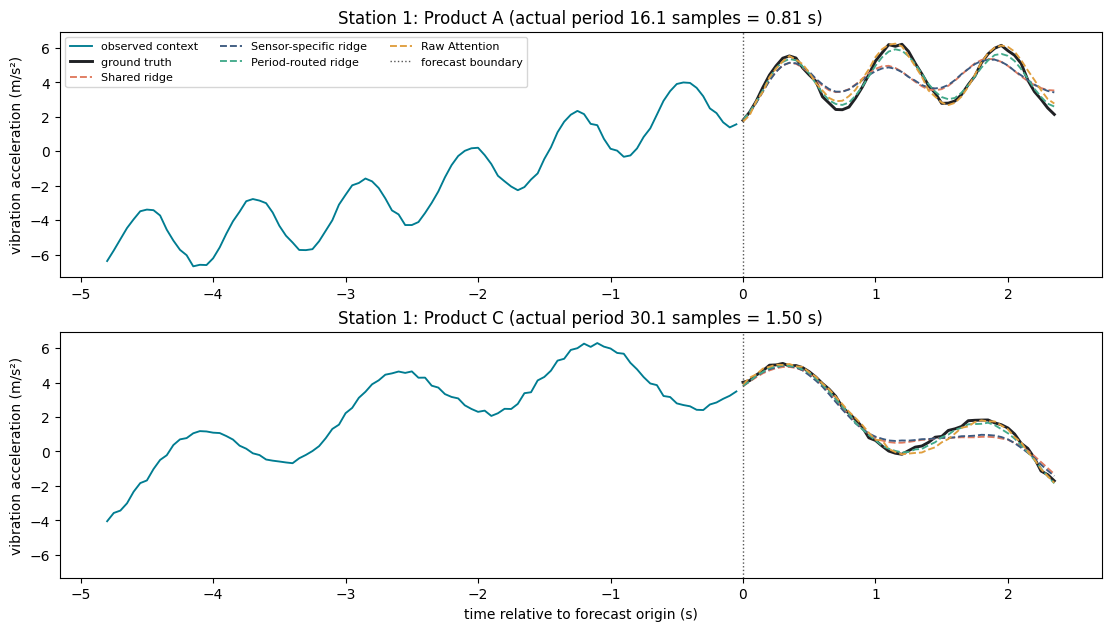
\includegraphics[width=\textwidth]{Images/curves.png}
    \caption{Forecasts for Station~1 under Products~A and~C. The black
    curve is the ground truth. Product~A has a period of approximately
    $16.1$ samples, while Product~C has a period of approximately
    $30.1$ samples. The fixed Shared Ridge mapping cannot adapt to both
    temporal patterns.}
    \label{fig:forecast_curves}
\end{figure}

Output 1.2 shows the resulting errors. Shared Ridge obtains RMSEs of
$0.779$ and $0.448$ for Products~A and~C, respectively. Sensor-specific
Ridge gives similar errors of $0.787$ and $0.436$. Period-routed Ridge
instead uses the estimated period to select the forecasting rule, reducing
the errors to $0.232$ and $0.150$. This suggests that the main limitation
is not simply linearity, but using the \emph{same temporal mapping} across
different production periods.

\subsubsection{Response 1.3. Context-dependent Attention mixing}
Attention also has fixed learned parameters $W_Q$, $W_K$, and $W_V$, but
its actual mixing weights depend on the input:
\begin{equation}
A(X)=
\operatorname{softmax}
\left(
\frac{(XW_Q)(XW_K)^{\top}}{\sqrt{d_h}}
\right),
\qquad
\operatorname{Attn}(X)=A(X)XW_V .
\end{equation}

Thus, while the learned parameters remain fixed, a new context produces
new query-key scores and therefore new mixing weights. Ridge always applies
the same $\hat{W}$, whereas Attention can change how information from the
96 positions is mixed.

Output 1.3 provides evidence of this context dependence. For the same
trained Attention model, the Product~A and Product~C windows have attention
weights that differ by a mean absolute difference of $0.003$ and a maximum
difference of $0.036$. This shows that the mixing operation changes with
the context, although it does not prove that Attention has explicitly
identified the physical production period.

The performance in Output 1.2 is consistent with this additional
flexibility. Raw Attention reduces the Shared Ridge RMSE from $0.779$ to
$0.297$ on Product~A and from $0.448$ to $0.198$ on Product~C, without
being explicitly given the period.

\paragraph{Summary.}
The key distinction is:
\[
\boxed{
\text{Shared Ridge: same }W\text{ for every context}
}
\]

\[
\boxed{
\text{Period-routed Ridge: estimate the period and choose }W
}
\]

\[
\boxed{
\text{Raw Attention: same }W_Q,W_K,W_V,\text{ but context-dependent mixing}
}
\]

The production period is therefore important because \textbf{station
identity alone does not determine the forecasting rule}. A single station
can operate at different paces, while Station~4 is completely unseen
during fitting, making a station-specific fitted matrix unavailable for
that station.


\subsection{Responses 2}

\subsubsection{ Selected width and what changed}

I implemented \texttt{SeriesDecomposition.forward} as a centered moving
average with replicate padding of $q=\lfloor m/2\rfloor$ samples at both
ends. The decomposition returns
\[
T=\operatorname{MA}_m(x), \qquad S=x-T,
\]
so that the original signal is exactly reconstructed as
\[
S+T=x.
\]
The width selected by the oracle diagnostic is
$\mathbf{m=41}$.

The purpose of the moving average is to separate the two different time
scales in the signal. The slow baseline changes over approximately
240 samples on the other hand the vibration has periods of only about 14-36
samples. A wide moving average would smooth out much of
the faster oscillation and left the slower structure in $T$, while the
remainder $S$ contained the variation that the moving average did not
absorb.

On the Station~2, Product~C context shown in Output~2.1, the effect of
the width is visible directly. At $m=17$, the trend still contained
noticeable oscillations from the vibration, and the remainder was
decreased (standard deviation $0.578$ m/s$^2$). As $m$ increased more of
the fast oscillation was removed from the trend. At $m=41$, the trend was
much smoother and mainly followed the slow drift (range approximately
$8$ m/s$^2$), while the remainder had a clearer oscillatory structure
(std.\ $1.572$ m/s$^2$).

As mentioned in reading note that remainder cannot not be interpreted as the ground truth vibration. It is just whatever the moving average coult not to absorb so it can still
have some slow structure and can also distort the peak of the
vibration. For example, with $m=41$ and an actual period of about
32 samples, the filter could subtract part of the periodic component and
slightly increase the corresponding remainder.

The boundary region also needs some caution. Because the filter uses
replicate padding near the two ends, the decomposition near the forecast
origin can behave slightly differently from the interior.

Most importantly, the right-hand diagnostic in Output~2.1 shows why the
decomposition is useful: the repetition score of the raw context is
relatively flat, whereas the width-$41$ remainder produces a much clearer
peak around the actual period of 32 samples.

\begin{figure}[H]
    \centering
    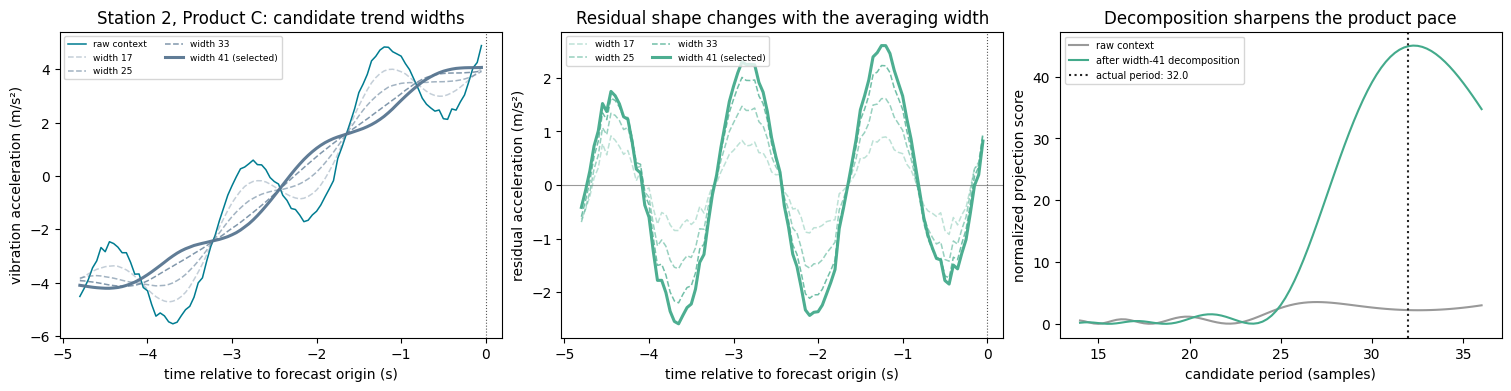
\includegraphics[width=\textwidth]{Images/width.png}
    \caption{Effect of the moving-average width on the decomposition and
    repetition structure. Increasing the width removes more of the fast
    oscillatory variation from the trend and leaves a clearer repeating
    component in the remainder.}
    \label{fig:width_selection}
\end{figure}


\subsubsection{Period recovery and selection of the width}

Output~2.2 measures whether the decomposition made the repeating
structure easier to recover. This was important because the raw context
contained both the slow base and the vibration. A slowly rising or falling
signal could look similar to a shifted copy of itself which can make a
shift-based repetition score misleading.

Every candidate width improved period recovery substantially. The fraction
of training contexts whose period is recovered within one sample increases
from $0.687$ for the raw representation to $0.980$--$0.998$ after
decomposition. At the same time, the median absolute period error falls
from $0.525$ samples to approximately $0.12$--$0.22$ samples.

The selected width, $m=41$, has the highest within-one-sample recovery rate
at $0.998$. Width $25$ has a slightly smaller median absolute error
($0.122$ versus $0.216$ samples), but its recovery rate is slightly lower
($0.989$ versus $0.998$). Thus, $m=41$ gives the most consistent period
recovery, although the difference between widths 25 and 41 is small.

This diagnostic is described as an oracle diagnostic because it uses the
known training periods to evaluate the quality of the decomposition. It is
used to choose the filter width; the true repeating component itself is
not provided to the forecasting model.

\begin{figure}[H]
    \centering
    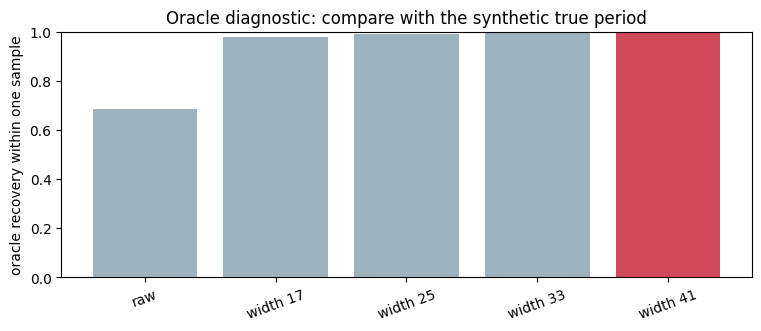
\includegraphics[width=\textwidth]{Images/diagnoctis.png}
    \caption{Period-recovery diagnostic for the raw representation and
    different moving-average widths. Decomposition substantially improves
    recovery of the known training periods.}
    \label{fig:diagnostic}
\end{figure}


\subsubsection{How decomposition changes the forecasting model}

Decomposition is not simply a preprocessing step applied once before
training. It changes the architecture of the Raw Attention forecaster.

First, the context is split into the remainder and trend:
\[
x \rightarrow (S,T).
\]

The remainder $S$ is sent through the Attention encoder, while the trend
$T$ is sent to a separate linear trend head:
\[
S \rightarrow \text{Attention encoder} \rightarrow \hat{S},
\qquad
T \rightarrow \text{linear head} \rightarrow \hat{T}.
\]

The final forecast is then
\[
\hat{y}=\hat{S}+\hat{T}.
\]

Thus, the linear head is responsible for forecasting the slow structure,
while Attention can focus on the faster repeating component. This is the
main architectural motivation for the decomposition.

Importantly, decomposition is also applied after each residual sublayer.
The resulting trend component is removed again before the next mixer sees
the representation. Therefore, slow structure introduced by a residual
connection does not simply accumulate through the Attention blocks.

\paragraph{Forecasting results.}

On the validation set, Attention plus decomposition reduces Raw
Attention's overall MSE from $0.188$ to $0.098$ (m/s$^2$)$^2$, a
$48\%$ reduction, with only $4{,}656$ additional parameters
($373{,}024$ versus $368{,}368$).

The improvement is present for every product and both station populations:

\begin{table}[htbp]
\centering
\caption{RMSE (m/s$^2$) of Raw Attention and Attention + decomposition
(Output 2.3).}
\label{tab:decomp_ablation}
\vspace{2mm}
\begin{tabular}{@{} l ccc ccc @{}}
\toprule
& \multicolumn{3}{c}{\textbf{Established}} &
  \multicolumn{3}{c}{\textbf{Held-out Station 4}} \\
\cmidrule(lr){2-4}\cmidrule(lr){5-7}
\textbf{Product} & Raw & Decomp. & Change &
\textbf{Raw} & \textbf{Decomp.} & \textbf{Change} \\
\midrule
A & 0.422 & \textbf{0.295} & $-30\%$
  & 0.702 & \textbf{0.401} & $-43\%$ \\
B & 0.464 & \textbf{0.353} & $-24\%$
  & 0.612 & \textbf{0.535} & $-13\%$ \\
C & 0.421 & \textbf{0.286} & $-32\%$
  & 0.645 & \textbf{0.433} & $-33\%$ \\
\bottomrule
\end{tabular}
\end{table}

The forecast examples illustratD where the improvement comes from. For
Station~4, Product~A, which has the largest improvement, the context
contains a substantial slow drift. Raw Attention produced a damped forecast
that gradually moved out of phase with the ground truth after approximately
$0.7$\,s. Attention plus decomposition followed the ground-truth oscillation
more closely across the forecast horizon.

For Station~4, Product~B, where the improvement is smallest, both models
capture the broad trend, but the decomposed forecast still develops a phase
lag that increases with the forecast horizon. In this case, the remaining
error is mainly in the repeating component rather than in the slow drift,
so removing the drift cannot eliminate that error.

Decomposition therefore addressed a specific limitation of the raw
representation: it prevents the slow drift from competing with the
repeating structure inside the Attention encoder. It does not explicitly
provide the period to the model, and it does not guarantee correct phase
prediction when the repeating component itself is difficult to forecast.
Period-routed Ridge still has the advantage of being explicitly routed by
the estimated production pace, with RMSEs of $0.166$ and $0.173$ for the
corresponding comparison.

\subsubsection{Why moving average is a sensible inductive bias}

A moving average is a sensible inductive bias for this
drift+repetition setting because the two components have very
different time scales. The slow baseline changes after
240 samples and the vibration repeats every roughly 14-36 samples.
Averaging over an suitable window can suppresses most of the
faster variation while retaining the slower structure/part.

This bias could fail if the slow component was changin abruptly or contained
important variation on the same time scale as the vibration. In that case
the moving average could smooth away useful information or mix the two
components. An alternative would be a learned decomposition or a
frequency-based filter which would make a different assumption about how
the slow and repeating components should be separated.

\subsubsection{If moving avg fails whats alternate method.}
The moving-average decomposition is appropriate here because the slow component
changes on a much longer timescale (about 240 samples) than the vibration
(periods of roughly 14-36 samples). However, this bias would fail if the
``slow'' component changed rapidly, for example if the baseline drift had
variations on a timescale comparable to the vibration period. In that case,
the moving average could incorrectly absorb part of the meaningful repetition
into the trend.

An alternative would be a \textbf{wavelet decomposition}. Instead of assuming
that slow structure can be isolated using a fixed temporal averaging window,
it assume that the signal can be separated into components at different
time scales. This would be more suitable if the frequency or period of the
repeating component changed substantially over time.

other alternative could be moving median filter. As it assumes the slow part is piecewise constant with occasional jumps rather than smooth. It would keep a sudden calibration jump sharp instead of spreading it over 41 samples, at the cost of being nonlinear and cancelling the vibration less cleanly than an average.

\subsection {Response 3}

\subsubsection*{Delay aggregation and verification}

I implemented \texttt{aggregate\_delays} according to Equation (6). For each selected
delay $\tau_j$, the operation retrieves the value $\tau_j$ samples earlier using
circular indexing and combines the retrieved values using the normalized weights
$\alpha_j$:

\begin{equation}
z_t =
\sum_{j=1}^{K}
\alpha_j v_{(t-\tau_j)\bmod L}.
\end{equation}

The indexing direction is therefore backward in time: a positive delay $\tau_j$
means that position $t$ retrieves the value at $t-\tau_j$. The modulo operation
makes the shift circular, so values that pass the beginning of the sequence wrap
around to the end.

The supplied aggregation check passed. For the worked example, the aggregated
values were $[35.0,15.0,25.0,25.0]$, exactly matching the expected values.
This verified both the numerical aggregation and the direction of the delay
indexing.


% \paragraph{Strongest recurrence and its relation to the period.}
% Output~3.2 shows a Station~2, Product~A run with actual period $P = 16.135$ samples.
% The residual correlation has its strongest peaks at delay 16 (nearest integer to $P$,
% correlation 0.896) and delay 32 (nearest integer to $2P = 32.27$, correlation 0.897),
% and the curve rises to a third peak of about 0.89 near delay 48 ($3P \approx 48.4$),
% at the upper edge of the delay band. These are the integer multiples of the period:
% a cycle that repeats every $P$ samples also repeats every $2P$ and $3P$. Halfway
% between them, at delays $\approx 24$ ($1.5P$) and $\approx 40$ ($2.5P$), the
% correlation reaches about $-0.92$, because the shifted copy places peaks on troughs.
% The peaks are nearly equal in height because the residual is dominated by one stable
% cycle with little noise.



\subsubsection{Recurrence in the signal}

Output 3.2 shows strong recurrence at delays of approximately one period and
two periods. For Station~2, Product~A, the actual period is
\[
P = 16.135 \text{ samples}.
\]
The strongest recurrence occurs at
\[
\tau=16 = P
\]
with a residual correlation of $0.896$. A second strong recurrence occurs at
\[
\tau=32 = 2P
\]
with a residual correlation of $0.897$. Thus, the signal becomes similar to
itself again after approximately one cycle and after two cycles.
This is exactly the type of temporal structure that the delay mixer is designed
to exploit. Rather than treating every position pair independently, it organizes
relationships according to their temporal displacement.

\begin{figure}[H]
    \centering
    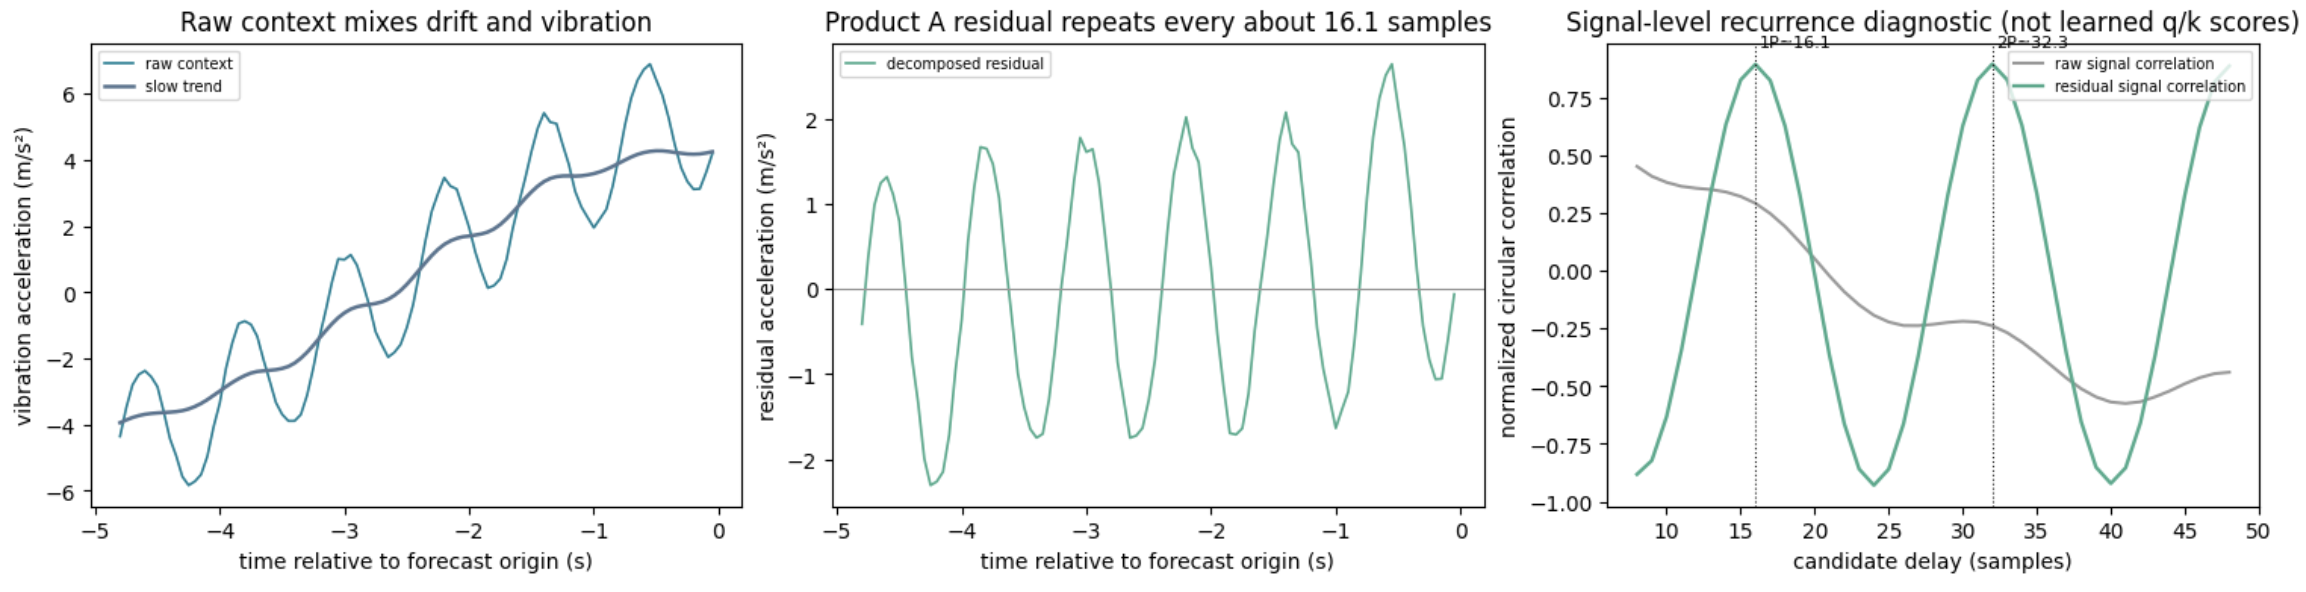
\includegraphics[width=1\linewidth]{Images/3.2.png}
    \caption{}
    \label{fig:3.2}
| \end{figure}

\paragraph{Strongest recurrence and its relation to the period.}
Output~3.2 shows a Station~2, Product~A run with actual period
$P = 16.135$ samples. The residual correlation has prominent positive
peaks at delays 16 (nearest integer to $P$, correlation $0.896$) and
32 (nearest integer to $2P = 32.27$, correlation $0.897$). A third
positive peak appears near delay 48, corresponding to
$3P \approx 48.4$. These peaks occur at approximately integer
multiples of the period because a periodic signal aligns with itself
after one, two, or three cycles.

The negative troughs near delays 24 ($\approx 1.5P$) and 40
($\approx 2.5P$) provide complementary evidence. At these
displacements, peaks in the original signal tend to align with
troughs in the shifted copy, producing strong negative correlation.
Thus, the recurrence pattern is organized around the operating
period and its multiples rather than around arbitrary positions.

\paragraph{Why decomposition makes the delay evidence cleaner.}
The raw context mixes a slow ramp with the repeating vibration. The ramp makes
nearby shifts look similar, so the raw correlation is highest at short delays
rather than clearly identifying the true period. At delay 16, for example, the
raw correlation is only about $0.30$.

After decomposition, the slow trend is removed and the residual is dominated by
the repeating vibration. Shifting it by the true period aligns peaks with peaks
and troughs with troughs, giving strong positive correlation. The residual
therefore shows clear peaks at approximately $P=16$, $2P=32$, and
$3P\approx48$, with correlations around $0.90$; shifts halfway between periods
align peaks with troughs and give strong negative correlation.

This supports the delay mixer's inductive bias: useful temporal relationships
can be organized by a small number of recurring delays. Decomposition makes
these delays easier to detect because the slow drift no longer dominates the
similarity.

Output~3.2 is a \emph{signal-level diagnostic}, not the trained mixer's scores.
The diagnostic uses the signal values directly, while the trained mixer scores
delays using learned query and key features.


\paragraph{When the delay assumption is wrong.}
Delay mixing assumes that useful temporal relationships occur at a few recurring
displacements. This assumption would fail for an \emph{isolated transient}, such
as a single impact or fault spike that occurs only once. There is no recurring
delay at which the event can be matched, so delay scores cannot identify it as a
repeating pattern. Also aggregation shifts the selected values across the
sequence, potentially creating artificial copies of the spike at other
positions. With circular shifting, these copies can even wrap around to the
start of the context. Thus, delay mixing could incorrectly treat a one-time
event as a recurring pattern.



\subsection{4 Response: Comparing Designs and Deploying}

\subsubsection{(a) Prior prediction}

I expected decomposition to help most when the slow trend is strong, because
removing the trend should make the repeating vibration easier for the mixer to
use. Output~3.2 showed that the slow trend can otherwise hide the true periodic
structure.




\subsubsection{(b) Validation results}
Both changes made Raw Attention better, but delay mixing made the bigger
difference (Table~\ref{tab:four_models}). On the established stations, RMSE
dropped from $0.443$ to $0.231$ with delay mixing and to $0.307$ with
decomposition; on Station~4, it dropped from $0.640$ to $0.336$ and $0.459$.
Using both gave the best neural model, Autoformer-inspired ($0.197$ and
$0.243$). The two gains overlap rather than add up: decomposition improved Raw
Attention by $31\%$ but the delay mixer by only $15\%$, likely because both
target the same drift-plus-repetition structure. The combined model is also not
best everywhere: on Station~4, Product~B it was the worst of the four ($0.382$
vs.\ $0.175$ for the raw delay mixer; Figure~\ref{fig:output41}).

\begin{table}[htbp]
\centering
\caption{Validation results (Outputs 4.1 and 1.1): RMSE (m/s$^2$) and MSE ((m/s$^2$)$^2$)
on the established stations and held-out Station~4, with parameter count and fitting time.}
\label{tab:four_models}
\vspace{2mm}
\resizebox{\textwidth}{!}{%
\begin{tabular}{@{}lcc|cc|rr@{}}
\toprule
& \multicolumn{2}{c|}{\textbf{Established}} &
  \multicolumn{2}{c|}{\textbf{Held-out Station 4}} &
  \textbf{Params} & \textbf{Fit (s)}\\
\textbf{Model} & RMSE & MSE & RMSE & MSE & & \\
\midrule
Shared ridge              & 0.767 & 0.588 & 0.876 & 0.767 & 4{,}608   & 0.003\\
Sensor-specific ridge     & 0.768 & 0.590 & --    & --    & 13{,}824  & 0.075\\
Period-routed ridge       & \textbf{0.166} & \textbf{0.028} & \textbf{0.173} & \textbf{0.030} & 59{,}904 & 0.013\\
\midrule
Raw Attention             & 0.443 & 0.196 & 0.640 & 0.409 & 368{,}368 & 79.0\\
Attention + decomposition & 0.307 & 0.094 & 0.459 & 0.210 & 373{,}024 & 93.4\\
Raw delay mixer           & 0.231 & 0.053 & 0.336 & 0.113 & 368{,}370 & 92.5\\
Autoformer-inspired       & 0.197 & 0.039 & 0.243 & 0.059 & 373{,}026 & 112.4\\
\bottomrule
\end{tabular}%
}
\end{table}

\begin{figure}[H]
\centering
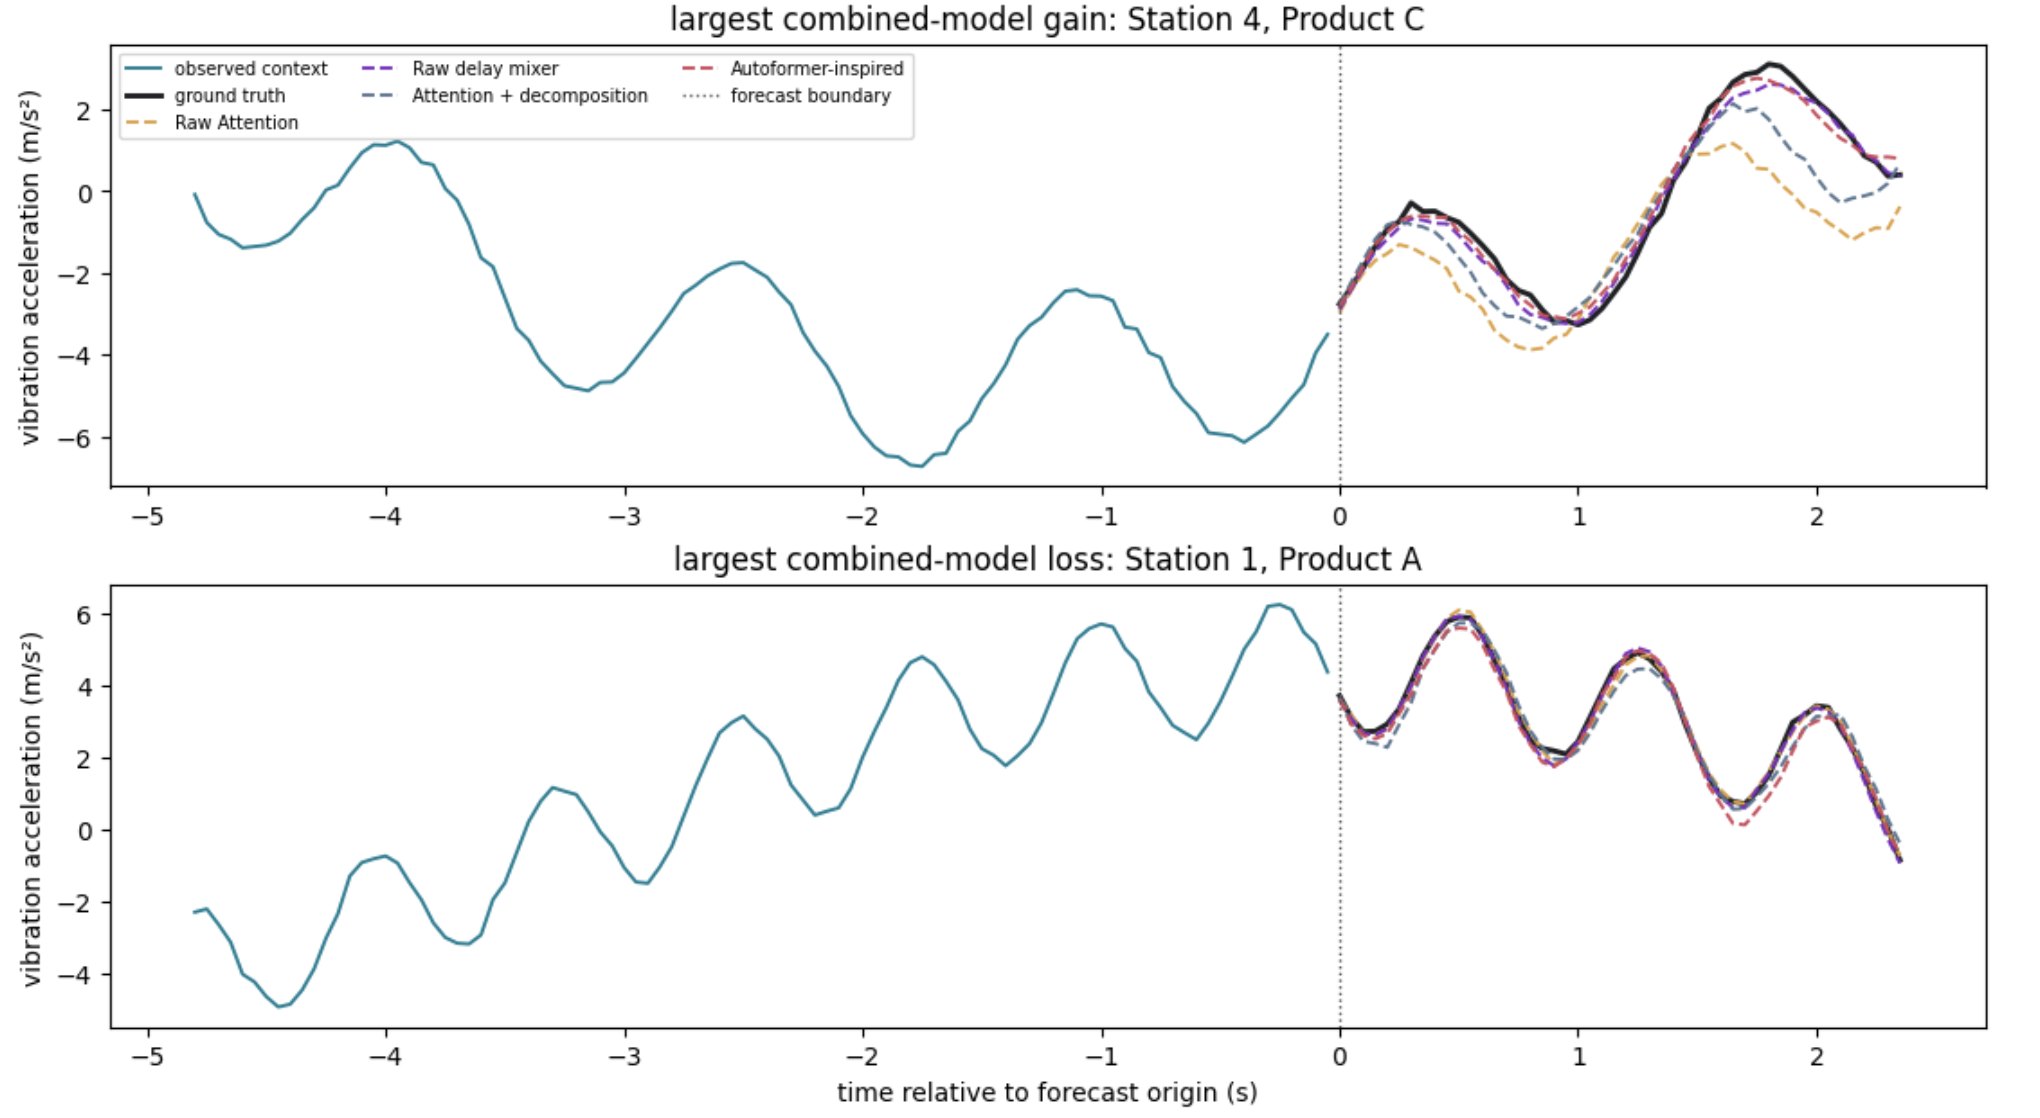
\includegraphics[width=\textwidth]{Images/4.2.png}
\caption{Contrasting forecast cases from Output~4.1. The top panel shows the
largest gain from the combined model on Station~4, Product~C. The delay-based
models track the repeating pattern much more closely than Raw Attention. The
bottom panel shows the largest combined-model loss on Station~1, Product~A,
where the raw delay mixer performs better than the two decomposed models.}
\label{fig:output41}
\end{figure}


\subsubsection{(c) Deployment choices}

I chose \textbf{period-routed ridge} for both the established stations and
Station~4. It had the lowest validation error ($0.166$ and $0.173$) with only
$59{,}904$ parameters and a $0.01$\,s fit, compared with about $370$k parameters
and $79$--$112$\,s for the neural models. It also suits the unseen station,
because it picks its forecasting rule from the estimated period, not the
station. Test RMSE ($0.161$ and $0.183$) agrees with validation.


\section{Task 2: Leaderboard Forecasting with Autoformer}

In this task I forecast the next 168 values of an anonymised univariate series with an Autoformer model. I implemented it in three stages. First I studied the series and the external file to understand what kind of signal I was dealing with. Second I built a preprocessing pipeline and a chronological validation rules that I could trust more than the leaderboard. Third I ran a series of experiments, each repeated over three random seeds to decide which inputs, features and settings would actually help. I am reporting all the sections below

%==========================================================================
\subsection{Understanding the data}

\subsubsection{The target series}

The training file contains 43,656 rows. Each row holds an integer time index, running from 1 to 43,656, and one observed value. Before doing anything else I checked the assumptions given in the assignment. The indices are consecutive with a step of one and there are no missing values, no value is negative and the test file covers exactly the indices 43,657 to 43,824. All of these checks passed.

Table~\ref{tab:stats} showing that the distribution is highly right-skewed. Half of all observations lie between 30 and 136, so the very large values are rare but they lie far away from the most of the data.

\begin{table}[h]
\centering
\caption{Summary statistics of the target over the 43,656 training steps.}
\label{tab:stats}
\begin{tabular}{lr}
\toprule
Statistic & Value \\
\midrule
Observations & 43,656 \\
Minimum & 0 \\
First quartile & 30 \\
Median & 73 \\
Mean & 98.2 \\
Third quartile & 136 \\
Maximum & 994 \\
Standard deviation & 90.8 \\
\bottomrule
\end{tabular}
\end{table}

Figure~\ref{fig:lastweek} showing a stretch of the series, the series does not move smoothly. It alternates between calm periods, in which the value stays around 10 to 20 for several days, and episodes in which it climbs to several hundred. The climb into an episode can be gradual. Around index 43,270, for example, the value rises from about 20 to almost 390 over roughly a day. The end of an episode, however, is often abrupt. Shortly after that peak the value fell from above 300 to below 30 within a few steps. This shape was the main difficulty of the task. A model that only looks at the recent past has no way of knowing when an episode will start or end, and a missed rise or a missed drop costs errors of several hundred units.

\begin{figure}[h]
\centering
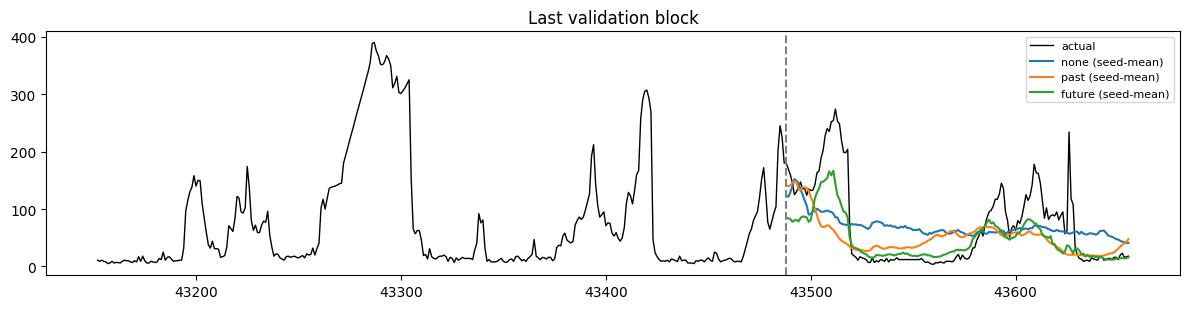
\includegraphics[width=\linewidth]{Images/fig_t2_01_last_val_week.pdf}
\caption{The last part of the training history (black). The dashed line marks the start of the last validation week. The coloured lines are the forecasts of the three covariate settings compared in Section~\ref{sec:covtiming}: no covariates, past covariates only, and past plus future covariates (each averaged over three seeds).}
\label{fig:lastweek}
\end{figure}

\subsubsection{Temporal dependence and periodic structure}

Because the timestamps were not given in the provided data so I had to recover the periodic structure from the data itself. Figure~\ref{fig:periodicity} shows the autocorrelation function (ACF) of $\log(1+y)$ and its periodogram.

The ACF falls from 1 to about 0.1 by lag 50 and is close to zero by lag 100. Beyond that point it only fluctuates within roughly $\pm 0.05$. In other words, the current value says a lot about the next few dozen steps, but almost nothing about what happens more than about 100 steps later. Since a forecast covers 168 steps, a large part of the horizon lies outside the memory of the series. This suggested that the past target alone could not produce a good forecast, and the experiments later confirmed it: without the external variables the validation RMSE stayed at 109.5, compared with 80.0 when their values over the horizon were included.

The periodogram showing one sharp peak at a period of 24 steps and a smaller peak at 12 steps. There is no peak at 168 steps, so the series has no weekly cycle. I also saw that peak is consistent with a yearly cycle.

These observations point to an hourly sampling interval. A dominant cycle of 24 steps with a 12-step harmonic a daily cycle in hourly data. The length of the full series supports this, because $43{,}824/24 = 1{,}826$ days, which is exactly five years of 365 days plus one leap day. The forecast horizon of 168 steps corresponds to one week, and the eight validation weeks that I hold out at the end of the training data come from the same season as the hidden test week.

Figure~\ref{fig:periodicity}(a) mark the lags that my automatic peak search returned as the strongest ACF peaks (lags 337, 505, 528 and 745). Their correlations are only between 0.05 and 0.07, and they do not share a common period, so they are noise. I did not use them, and I relied on the periodogram instead.

\begin{figure}[h]
\centering
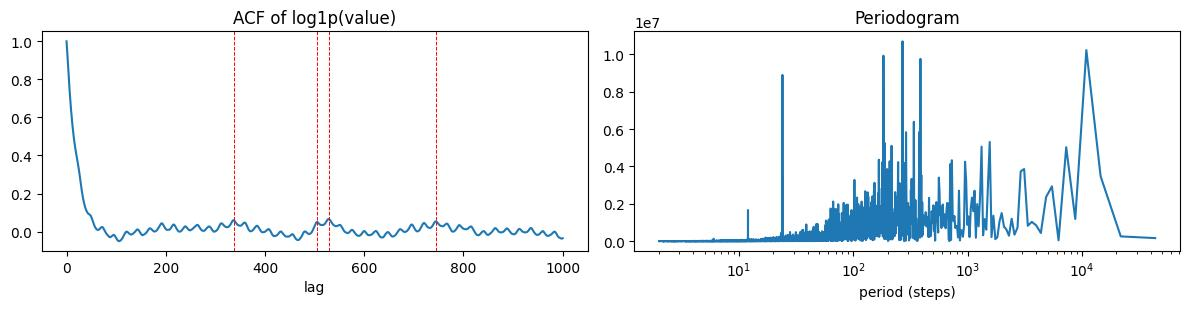
\includegraphics[width=\linewidth]{Images/fig_t2_02_periodicity.pdf}
\caption{(a) Autocorrelation of $\log(1+y)$ up to lag 1,000. (b) Periodogram, plotted against the period in steps. The sharp peaks at 24 and 12 steps are the daily cycle and its harmonic.}
\label{fig:periodicity}
\end{figure}

This analysis shaped three design decisions. First, the daily cycle is real but explains only a small part of the variance, so the periodic signal that Auto-Correlation can exploit is weak. Second, I set the moving-average window of the series decomposition to 25 steps, which is about one day. With this window the ``trend'' component represents the daily average level and the ``seasonal'' component represents the shape within the day. Third, because the past target carries little information beyond about 100 steps, the external variables had to supply the information for most of the horizon.

\subsubsection{External variables}

The file \texttt{optional\_external\_data.csv} contains 43,824 rows, so it covers the 168 test positions as well as the whole history. It has ten variables. Six of them, \texttt{feature\_A} to \texttt{feature\_F}, are continuous. The other four, \texttt{feature\_G} to \texttt{feature\_J}, are binary. I checked that exactly one of the four binary variables equals one at every time step, which means they are a one-hot encoding of a single categorical variable with four states. None of the ten variables has missing values.

The most important property of this file is its timing. The variables are measured on the same clock as the target, and their values are available for the forecast horizon too. If the target responds mainly to the conditions at the same moment, then the future values of these variables carry exactly the information that the past target lacks.The result is reported in Section~\ref{sec:covtiming}.


\subsection{Preprocessing}

\paragraph{Validation split first.} I fixed the validation split before fitting any statistics, so that no information from the validation period could leak into training. The last 1,344 steps of the training data (eight weeks, indices 42,313 to 43,656) were held out. Every scaler is fitted only on the steps before that point.

\paragraph{Target transformation and scaling.} Because the target is heavy-tailed, in my first pipeline I applied $\log(1+y)$ and then standardised the result to zero mean and unit variance. The log compressed the large episodes and made training more stable. To produce a forecast the model output was de-standardised, transformed back with $\exp(\cdot)-1$, and clipped at zero, since the target is non-negative. Later experiments showed that the log transform biases the forecasts downward and increased RMSE (Section~\ref{sec:target}), so the final pipeline standardised the raw values. In both versions the forecast is clipped to the range $[0, 994]$, where 994 is the largest value observed in training. 

\paragraph{External variables.} The six continuous variables were standardised with the same training-period statistics as the target. The four binary variables are left as 0 and 1, because they already have a clear and bounded scale.

\paragraph{Window construction.} Each training example is defined by a forecast origin $o$. The encoder receives the 336 target values before the origin, which is two weeks of history. The decoder covers 336 positions starting 168 steps before the origin. Following the original Autoformer, the decoder input is built from the series decomposition of the encoder window. Its first half holds the seasonal and trend components of the last 168 observed values, which give the decoder a warm start. Its second half is the forecast horizon, where the target is unknown, so the seasonal part is set to zero and the trend part to the mean of the encoder window. The training target is the 168 values starting at the origin. I used every possible origin (stride 1) whose target ends before the validation period, which gives 41,809 training windows. The final refit on the full history uses 43,153 windows. For validation I used 50 forecast origins, one every 24 steps across the held-out region, and additionally the eight non-overlapping weekly origins to measure how much the error varies from one week to the next.

\paragraph{How the external variables enter the model.} The external variables enter as ``marks'', which is the same mechanism the original Autoformer uses for calendar features. At every time step a linear layer maps the vector of external variables to the model dimension, and the result is added to the embedding of the target value. The encoder receives the external variables for its 336 past steps. The decoder receives them for all of its 336 positions, including the 168 future steps. This means that for every step of the horizon the decoder knows the external conditions, even though it does not know the target. In the ``past only'' setting of the ablation, the future part of the decoder's external input is set to zero.

\paragraph{Post-processing.} The final forecast is the average of the forecasts of three models trained with different seeds, clipped to $[0, 994]$ as described above.

%==========================================================================
\subsection{Feature engineering}
\label{sec:features}

All new features are computed only from the external file or from the time index. None of them uses the target, so they are available for all 43,824 steps, including the forecast horizon, and they cannot leak information about the values being predicted. I built two groups of features.

\paragraph{Time-phase features.} Autoformer was designed to receive calendar information, such as the hour of the day or the month, through its marks. The anonymisation removed this information. I rebuilt it from the periods found in the data analysis by adding four features: $\sin(2\pi t/24)$ and $\cos(2\pi t/24)$ for the daily cycle, and $\sin(2\pi t/8766)$ and $\cos(2\pi t/8766)$ for the yearly cycle, where 8,766 is $365.25 \times 24$. A sine and cosine pair encodes the position on a cycle smoothly, and a linear layer can learn any phase shift from it. These features rely on the assumption that the sampling is hourly and that the phase of each cycle stays stable over time.

\paragraph{Dynamics features.} The episodes in Figure~\ref{fig:lastweek} start and end abruptly. Such transitions are more likely to be linked to \emph{changes} in the external conditions than to their level alone. To make these changes explicit, I added two features for each of the six continuous variables $x$. The first is the change over six steps, $\Delta_6 x_t = x_t - x_{t-6}$, with the first six steps set to zero. The second is a centred rolling mean over 24 steps, which summarises the daily average conditions with less noise than the raw value. The centred window uses values up to 12 steps ahead. This is allowed, because the external file is known up to the end of the horizon, and at the very end of the file the window simply becomes shorter. This group adds twelve features.

With these features the model receives 14 inputs (time phase), 22 inputs (dynamics) or 26 inputs (both) instead of the original ten. Each additional input adds only $2 \times 32 = 64$ parameters, one weight per model dimension in the encoder mark layer and one in the decoder mark layer. The final model with dynamics features therefore has 31,041 parameters instead of 30,273.

%==========================================================================

\subsection{Standard vs.\ Adapted Autoformer}

\begin{figure}[H]
\centering
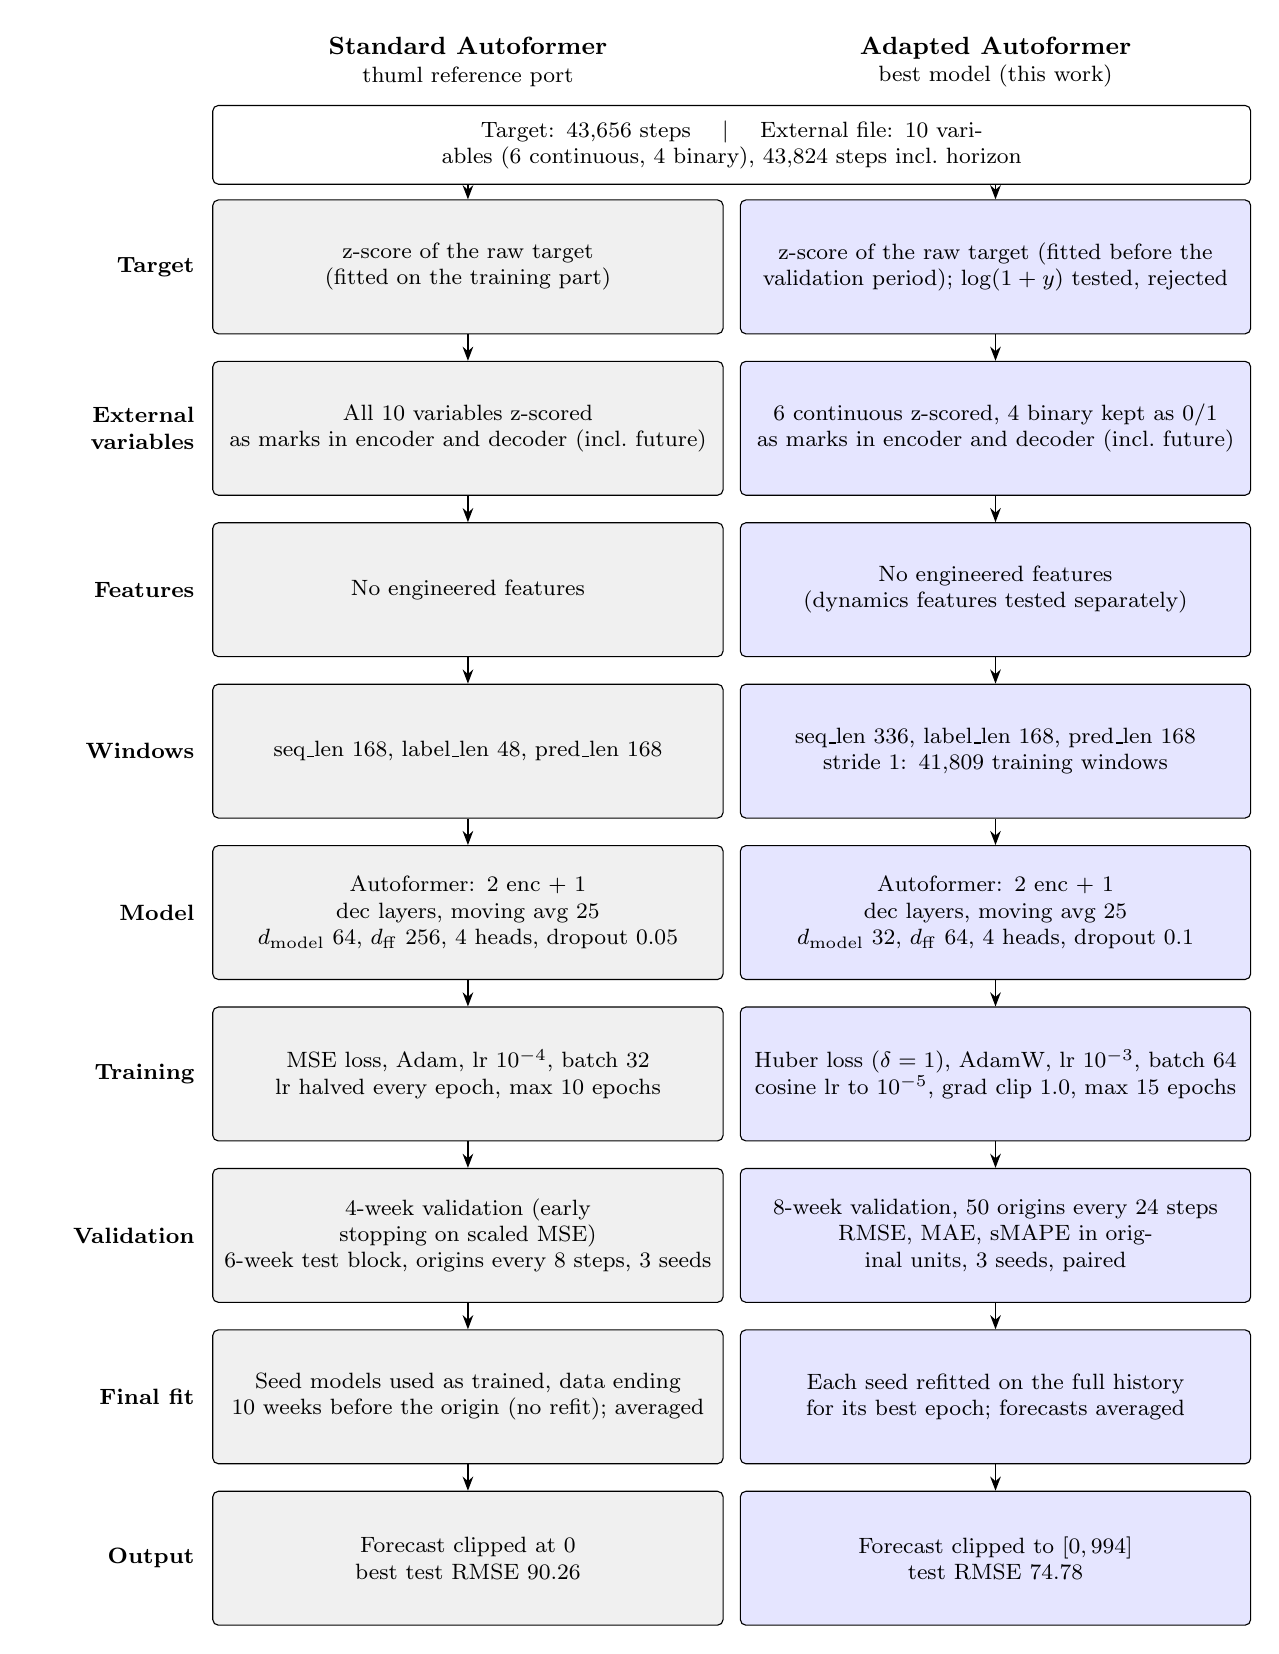
\begin{tikzpicture}[
  font=\footnotesize,
  box/.style={draw, rounded corners=2pt, align=center, text width=6.2cm, minimum height=1.7cm, inner sep=4pt},
  std/.style={box, fill=gray!12},
  ada/.style={box, fill=blue!10},
  stage/.style={align=right, text width=2.0cm, anchor=east, font=\footnotesize\bfseries},
  arr/.style={-{Stealth[length=1.8mm]}, semithick}
]
\def\xL{4.4}
\def\xR{11.1}

% column headers
\node[align=center, font=\small\bfseries] at (\xL, 2.0) {Standard Autoformer\\[-1pt]{\footnotesize\normalfont thuml reference port}};
\node[align=center, font=\small\bfseries] at (\xR, 2.0) {Adapted Autoformer\\[-1pt]{\footnotesize\normalfont best model (this work)}};

% shared input
\node[box, text width=12.9cm, minimum height=1.0cm, fill=white] (D) at ({(\xL+\xR)/2}, 0.95)
  {Target: 43,656 steps \quad $|$ \quad External file: 10 variables (6 continuous, 4 binary), 43,824 steps incl.\ horizon};

% rows
\node[stage] at (\xL-3.35, -0.60)  {Target};
\node[std] (L1) at (\xL, -0.60)  {z-score of the raw target\\(fitted on the training part)};
\node[ada] (R1) at (\xR, -0.60)  {z-score of the raw target (fitted before the\\validation period); $\log(1+y)$ tested, rejected};

\node[stage] at (\xL-3.35, -2.65)  {External variables};
\node[std] (L2) at (\xL, -2.65)  {All 10 variables z-scored\\as marks in encoder and decoder (incl.\ future)};
\node[ada] (R2) at (\xR, -2.65)  {6 continuous z-scored, 4 binary kept as 0/1\\as marks in encoder and decoder (incl.\ future)};

\node[stage] at (\xL-3.35, -4.70)  {Features};
\node[std] (L3) at (\xL, -4.70)  {No engineered features};
\node[ada] (R3) at (\xR, -4.70)  {No engineered features\\(dynamics features tested separately)};

\node[stage] at (\xL-3.35, -6.75)  {Windows};
\node[std] (L4) at (\xL, -6.75)  {seq\_len 168, label\_len 48, pred\_len 168};
\node[ada] (R4) at (\xR, -6.75)  {seq\_len 336, label\_len 168, pred\_len 168\\stride 1: 41,809 training windows};

\node[stage] at (\xL-3.35, -8.80)  {Model};
\node[std] (L5) at (\xL, -8.80)  {Autoformer: 2 enc + 1 dec layers, moving avg 25\\$d_{\mathrm{model}}$ 64, $d_{\mathrm{ff}}$ 256, 4 heads, dropout 0.05};
\node[ada] (R5) at (\xR, -8.80)  {Autoformer: 2 enc + 1 dec layers, moving avg 25\\$d_{\mathrm{model}}$ 32, $d_{\mathrm{ff}}$ 64, 4 heads, dropout 0.1};

\node[stage] at (\xL-3.35, -10.85) {Training};
\node[std] (L6) at (\xL, -10.85) {MSE loss, Adam, lr $10^{-4}$, batch 32\\lr halved every epoch, max 10 epochs};
\node[ada] (R6) at (\xR, -10.85) {Huber loss ($\delta=1$), AdamW, lr $10^{-3}$, batch 64\\cosine lr to $10^{-5}$, grad clip 1.0, max 15 epochs};

\node[stage] at (\xL-3.35, -12.90) {Validation};
\node[std] (L7) at (\xL, -12.90) {4-week validation (early stopping on scaled MSE)\\6-week test block, origins every 8 steps, 3 seeds};
\node[ada] (R7) at (\xR, -12.90) {8-week validation, 50 origins every 24 steps\\RMSE, MAE, sMAPE in original units, 3 seeds, paired};

\node[stage] at (\xL-3.35, -14.95) {Final fit};
\node[std] (L8) at (\xL, -14.95) {Seed models used as trained, data ending\\10 weeks before the origin (no refit); averaged};
\node[ada] (R8) at (\xR, -14.95) {Each seed refitted on the full history\\for its best epoch; forecasts averaged};

\node[stage] at (\xL-3.35, -17.00) {Output};
\node[std] (L9) at (\xL, -17.00) {Forecast clipped at 0\\best test RMSE 90.26};
\node[ada] (R9) at (\xR, -17.00) {Forecast clipped to $[0, 994]$\\test RMSE 74.78};

% arrows
\draw[arr] (D.south -| L1.north) -- (L1.north);
\draw[arr] (D.south -| R1.north) -- (R1.north);
\foreach \i in {1,...,8} {
  \pgfmathtruncatemacro{\j}{\i+1}
  \draw[arr] (L\i.south) -- (L\j.north);
  \draw[arr] (R\i.south) -- (R\j.north);
}
\end{tikzpicture}
\caption{Standard and adapted Autoformer pipelines, stage by stage.}
\label{fig:pipeline}
\end{figure}
%==========================================================================

\subsection{Experimental setup}
\label{sec:setup}

\paragraph{Model and training.} The model is an Autoformer encoder--decoder adapted from the official implementation (\url{https://github.com/thuml/Autoformer}), with the settings shown in Figure~\ref{fig:pipeline}. I started with $d_{\text{model}} = 64$ (117,889 parameters) and later reduced it to $d_{\text{model}} = 32$ (30,273 parameters, or 31,041 with the dynamics features). Training used the Huber loss and AdamW with a cosine learning-rate schedule. Each run lasts at most 15 epochs, stops once the validation RMSE has not improved for three epochs, and kept the weights of its best epoch.

\paragraph{How I compared configurations.} Every configuration was trained with three seeds, and I reported the mean and standard deviation of its validation RMSE, MAE and sMAPE. To compare two configurations, I took the RMSE difference seed by seed, since runs with the same seed share their initialisation and batch order. I also counted how many seeds and how many of the 50 validation windows improved. In addition, I report the 3-seed ensemble, the average of the three forecasts, because that is the form I submit. Choosing the best epoch on the validation set makes all numbers slightly optimistic, but it does so equally for every configuration, so the comparisons stay fair.

%==========================================================================
\subsection{Results without engineered features}

\subsubsection{Do the external variables help, and which part of them?}
\label{sec:covtiming}

I compared three settings with the same model: no external variables, external variables for the past only, and external variables for the past and for the forecast horizon. Table~\ref{tab:covtiming} and Figure~\ref{fig:covablation} show the results, evaluated on the same 50 validation windows.

\begin{table}[h]
\centering
\caption{Covariate timing (log target, $d_{\text{model}} = 64$). RMSE, MAE and sMAPE are means $\pm$ standard deviation over three seeds. $\Delta$RMSE is the seed-by-seed difference to the model without covariates.}
\label{tab:covtiming}
\small
\resizebox{\linewidth}{!}{%
\begin{tabular}{lcccccc}
\toprule
Setting & RMSE & MAE & sMAPE (\%) & 3-seed ensemble RMSE & $\Delta$RMSE & Seeds better \\
\midrule
Persistence (last value) & 155.4 & 114.0 & 105.0 & -- & -- & -- \\
Seasonal naive (period 24) & 145.5 & 106.3 & 107.3 & -- & -- & -- \\
No covariates & $109.5 \pm 4.8$ & $81.5 \pm 4.0$ & $95.1 \pm 2.3$ & 107.7 & -- & -- \\
Past covariates only & $120.3 \pm 3.1$ & $85.2 \pm 3.2$ & $96.0 \pm 0.9$ & 117.7 & $+10.8 \pm 6.9$ & 0/3 \\
Past + future covariates & $\mathbf{80.0 \pm 3.6}$ & $\mathbf{51.1 \pm 2.6}$ & $\mathbf{58.6 \pm 1.7}$ & \textbf{76.5} & $\mathbf{-29.6 \pm 7.8}$ & \textbf{3/3} \\
\bottomrule
\end{tabular}}
\end{table}

\begin{figure}[H]
\centering
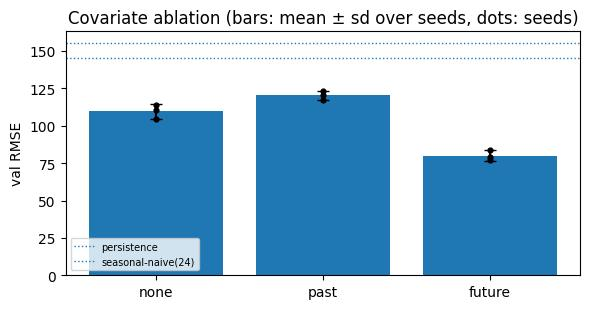
\includegraphics[width=0.6\linewidth]{Images/fig_t2_03_covariate_ablation.pdf}
\caption{Validation RMSE for the three covariate settings. Bars show the mean over three seeds, dots show the individual seeds, and the dotted lines mark the persistence and seasonal-naive baselines.}
\label{fig:covablation}
\end{figure}

Without external variables, the model reached an RMSE of 109.5. This was clearly better than the two naive baselines, so the model didnot learn the general level and the daily shape. It was still a weak forecast, and the learning curves in Figure~\ref{fig:learning} explain why. The training RMSE kept falling, but the validation RMSE stayed between about 105 and 120 for all three seeds. The limit is the information available to the model, not the optimisation. This matched the fast decay of the ACF.

Giving the model the past values of the external variables made the forecast \emph{worse}. The RMSE rose by $10.8 \pm 6.9$, all three seeds became worse, and the new model had the lower error in only 22\% of the validation windows. The learning curves show the reason. The best epoch was already reached after one to three epochs, and after that the training RMSE kept falling while the validation RMSE rose. This is overfitting. Past external values carry little information about a horizon of a week, and the extra inputs give the model more ways to fit noise in the training windows.

Giving the model the external variables over the forecast horizon as well changed the picture completely. The RMSE fell to 80.0, an improvement of $29.6 \pm 7.8$ over the model without covariates. The improvement held for all three seeds and in 89\% of the validation windows, and the effect is about four times larger than its spread across seeds. MAE fell from 81.5 to 51.1 and sMAPE from 95.1\% to 58.6\%. This was the largest single effect in the whole study. Figure~\ref{fig:lastweek} shows what it means in practice. In the last validation week, the model without covariates only follows the general level of the series. The model with future covariates reproduces the timing of the episode at the start of the week, the sharp drop that ends it, and the calm period that follows.

My conclusion is that the value of the external file comes almost entirely from its values during the forecast horizon. This is consistent with a target that responds to the conditions at the same moment rather than to earlier conditions. From this point on, every model receives the external variables over both the past and the horizon.

\begin{figure}[h]
\centering
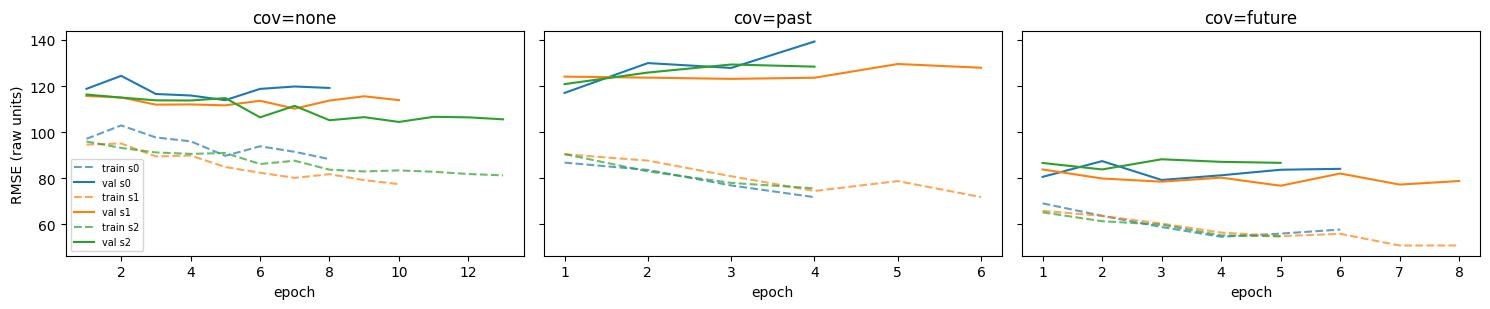
\includegraphics[width=\linewidth]{Images/fig_t2_04_learning_curves.pdf}
\caption{Training RMSE (dashed) and validation RMSE (solid) per epoch for each seed, for the three covariate settings. Runs end at different epochs because of early stopping.}
\label{fig:learning}
\end{figure}

\subsubsection{Where the external variables should enter, and which ones matter}

Next I tested two questions about the external variables in the second session, using the past-plus-future model as the reference. Table~\ref{tab:design} reports the results.

The first question was where in the architecture the variables should enter. In the ``decoder only'' variant, the encoder no longer receives the external variables, while the decoder still receives them for the label part and the horizon. This variant was worse by $8.7 \pm 9.0$ and lost on all three seeds. So the external variables are useful in the encoder, but only together with their future values in the decoder. A plausible explanation is that the encoder can relate the past target to the past conditions inside the same window, which helps the decoder interpret the future conditions. On their own, past values did not help at all, as the previous experiment showed.

The second question was which variables carry the signal. Using only the six continuous variables gave almost the same result as using all ten ($-1.1 \pm 5.4$, which is well within the noise). Using only the four binary variables was clearly worse ($+10.8 \pm 5.2$, all seeds worse), although it was still much better than using no external variables at all (109.5). So the binary variables carry some information on their own, but nearly all of the signal is in the continuous variables, and once those are present the binary variables add little. Because dropping the binary variables did not give a reliable improvement, I kept all ten.

\begin{table}[h]
\centering
\caption{Design experiments without engineered features (second session). $\Delta$RMSE is the seed-by-seed difference to the reference. ``Windows better'' is the fraction of the 50 validation windows in which the variant has the lower error.}
\label{tab:design}
\small
\resizebox{\linewidth}{!}{%
\begin{tabular}{lcccccc}
\toprule
Variant & RMSE & MAE & sMAPE (\%) & $\Delta$RMSE & Seeds / windows better & Parameters \\
\midrule
Reference (log target, $d_{\text{model}}$ 64) & $79.0 \pm 2.3$ & -- & -- & -- & -- & 117,889 \\
Covariates in decoder only & $87.7 \pm 6.7$ & 55.1 & 59.5 & $+8.7 \pm 9.0$ & 0/3, 51\% & 117,249 \\
Continuous covariates only & $77.9 \pm 3.2$ & 51.1 & 61.6 & $-1.1 \pm 5.4$ & 2/3, 58\% & 117,377 \\
Binary covariates only & $89.9 \pm 5.4$ & 57.5 & 65.3 & $+10.8 \pm 5.2$ & 0/3, 30\% & 117,121 \\
Raw target & $73.7 \pm 4.9$ & 55.9 & 77.2 & $-5.3 \pm 2.6$ & 3/3, 60\% & 117,889 \\
$d_{\text{model}}$ 32 (log target) & $76.1 \pm 4.2$ & 46.6 & 54.4 & $-3.0 \pm 5.8$ & 2/3, 54\% & 30,273 \\
\textbf{Raw target + $d_{\text{model}}$ 32} & $\mathbf{71.5 \pm 2.0}$ & 53.0 & 83.4 & $\mathbf{-7.6 \pm 2.5}$ & \textbf{3/3, 60\%} & \textbf{30,273} \\
\bottomrule
\end{tabular}}
\end{table}

\subsubsection{Target transformation and model size}
\label{sec:target}

The last two questions of this stage concerned the target transformation and the size of the model. I tested them as a two-by-two design, so that each effect could be checked at both levels of the other. Table~\ref{tab:twobytwo} reports the 3-seed ensembles.

\begin{table}[h]
\centering
\small
\setlength{\tabcolsep}{5pt} % Adjusts horizontal column spacing
\caption{Target transformation $\times$ model size. RMSE per seed is the mean over the three single models. The remaining columns refer to the 3-seed ensemble.}
\label{tab:twobytwo}
\begin{tabular}{llcccc}
\toprule
& & Single & \multicolumn{3}{c}{Ensemble} \\
\cmidrule(lr){3-3} \cmidrule(lr){4-6}
Target & Model size & RMSE & RMSE & MAE & sMAPE (\%) \\
\midrule
$\log(1+y)$ & $d_{\text{model}}$ 64 & 79.0 & 74.8 & 46.9 & 55.2 \\
raw         & $d_{\text{model}}$ 64 & 73.7 & 70.7 & 53.7 & 71.1 \\
$\log(1+y)$ & $d_{\text{model}}$ 32 & 76.1 & 72.9 & \textbf{44.3} & \textbf{51.5} \\
raw         & $d_{\text{model}}$ 32 & \textbf{71.5} & \textbf{67.1} & 49.5 & 71.3 \\
\bottomrule
\end{tabular}
\end{table}
The raw target lowered the RMSE at both model sizes. With $d_{\text{model}} = 64$ the gain was $5.3 \pm 2.6$, and with $d_{\text{model}} = 32$ it was $4.6 \pm 3.5$. Both gains held for all three seeds. The reason lies in the transformation itself. A model trained on $\log(1+y)$ learns to predict a central value on the log scale, and transforming that value back gives something close to the \emph{median} of the target, not its mean. For a right-skewed target the median is lower than the mean. RMSE, however, is minimised by the mean. The log-trained forecasts are therefore systematically too low during the episodes, which is exactly where the largest squared errors occur. Training on the raw scale removes this bias.

The raw target has a price, and it shows clearly in the other two metrics. MAE and sMAPE became worse. With $d_{\text{model}} = 32$, for example, the ensemble sMAPE rose from 51.5\% to 71.3\%. The raw-trained model tends to overestimate in calm periods. When the true value is 10, a forecast of 25 is a small absolute error but a large relative error, and sMAPE punishes relative errors heavily. The raw-trained model can also produce negative values that are clipped to zero, and a forecast of zero against a small positive value counts as a 200\% error in sMAPE. The three metrics therefore disagree in an informative way. The log target is better for relative accuracy at low values, while the raw target is better for accuracy during the episodes. Because the leaderboard ranks submissions by RMSE, I chose the raw target.

The smaller model was at least as good as the larger one at both target settings ($-3.0 \pm 5.8$ with the log target and $-2.2 \pm 4.9$ with the raw target, two of three seeds better in each case). It uses a quarter of the parameters and trains about twice as fast (19 instead of 36 seconds per epoch). The combination of raw target and small model was also the most stable configuration. Its spread across seeds was the smallest of all variants (2.0), and its best epochs (11, 10 and 5) came later than those of the larger raw-target model (1, 1 and 11). This made the number of epochs for the final refit more trustworthy.

\subsubsection{Result of the best model without engineered features}
\label{sec:rawsmall}

The best configuration without engineered features is therefore the raw target with $d_{\text{model}} = 32$, using all ten external variables in the encoder and the decoder. I call it \emph{raw-small}. Its single models reach $71.5 \pm 2.0$ on validation, and its 3-seed ensemble reaches an RMSE of 67.1, an MAE of 49.5 and an sMAPE of 71.3\%.

To produce the forecast, I refitted each of the three seeds on the full history for the number of epochs at which it had performed best on validation (11, 10 and 5 epochs), using the same learning-rate schedule. Table~\ref{tab:refit} lists the training metrics at the end of each refit. The training RMSE lies between 55 and 61, which is moderately below the validation RMSE of the single models, so the generalisation gap is modest. This ensemble became submission \#3, with $P = 3 \times 30{,}273 = 90{,}819$ parameters and $E = 61$ epochs (35 epochs in the three validation runs plus 26 epochs of refitting). On the leaderboard it reached an RMSE of 74.78, an MAE of 49.66 and an sMAPE of 60.40\%, which is my best result. Figure~\ref{fig:submitted} shows the forecast.

\begin{table}[h]
\centering
\caption{Training metrics at the end of the full-history refit for the members of the submitted ensembles. They are evaluated on one training window every 168 steps over the whole history.}
\label{tab:refit}
\small
\begin{tabular}{llcccc}
\toprule
Submission & Member & Refit epochs & Train RMSE & Train MAE & Train sMAPE (\%) \\
\midrule
raw-small & seed 0 & 11 & 61.1 & 45.4 & 60.1 \\
 & seed 1 & 10 & 54.7 & 38.5 & 56.3 \\
 & seed 2 & 5 & 59.8 & 41.7 & 57.4 \\
\midrule
fe-dyn & seed 0 & 6 & 53.9 & 37.8 & 58.6 \\
 & seed 1 & 3 & 56.2 & 38.3 & 60.2 \\
 & seed 2 & 1 & 67.2 & 44.5 & 63.5 \\
\bottomrule
\end{tabular}
\end{table}

\begin{figure}[h]
\centering
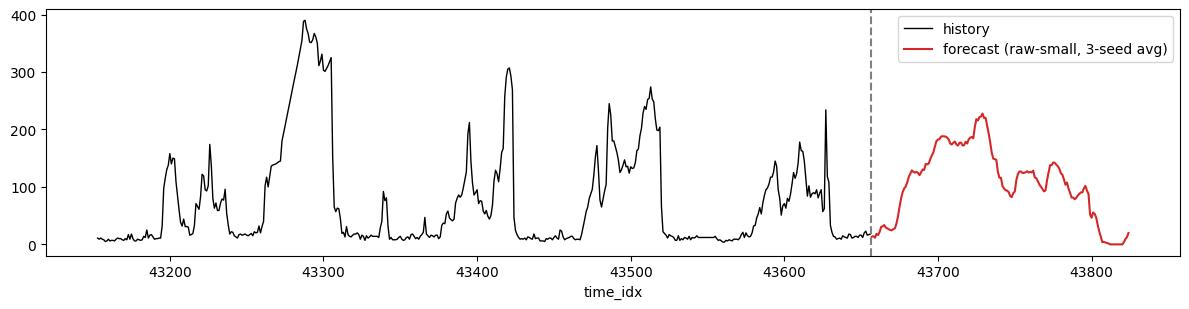
\includegraphics[width=\linewidth]{Images/fig_t2_05_submitted_forecast.pdf}
\caption{ the 3-seed raw-small forecast for indices 43,657 to 43,824 (red), after the last two weeks of the training history (black).}
\label{fig:submitted}
\end{figure}



%==========================================================================
\subsection{Experiments with engineered features}

I added the engineered features from Section~\ref{sec:features} to raw-small and compared each variant with it seed by seed (Table~\ref{tab:fe}). In short, the dynamics features improved the validation scores, but the gain did not carry over to the test week, so the best submitted model uses no engineered features.

\begin{table}[h]
\centering
\caption{Experiments with engineered features. All variants use the raw target and $d_{\text{model}} = 32$ unless stated otherwise. $\Delta$RMSE is the seed-by-seed difference to the reference given in the last column.}
\label{tab:fe}
\small
\resizebox{\linewidth}{!}{%
\begin{tabular}{lccccccl}
\toprule
Variant & RMSE per seed & Ensemble RMSE & MAE & sMAPE (\%) & $\Delta$RMSE & Seeds better & Reference \\
\midrule
raw-small (no new features) & $71.5 \pm 2.0$ & 67.1 & 49.5 & 71.3 & -- & -- & -- \\
+ time phase & $71.4 \pm 5.2$ & 68.9 & 50.8 & 68.5 & $-0.1 \pm 5.6$ & 2/3 & raw-small \\
\textbf{+ dynamics (fe-dyn)} & $\mathbf{66.4 \pm 1.7}$ & \textbf{63.5} & \textbf{47.4} & 69.4 & $\mathbf{-5.1 \pm 1.5}$ & \textbf{3/3} & raw-small \\
+ time phase + dynamics & $68.5 \pm 2.9$ & 65.9 & 49.4 & 68.6 & $+2.1 \pm 3.7$ & 1/3 & fe-dyn \\
fe-dyn with MSE loss & $71.3 \pm 3.1$ & 68.1 & 51.8 & 72.3 & $+5.0 \pm 2.5$ & 0/3 & fe-dyn \\
fe-dyn with log target & $75.4 \pm 4.5$ & -- & -- & -- & $-0.7 \pm 5.8$ & 1/3 & log, no new features \\
\bottomrule
\end{tabular}}
\end{table}

\paragraph{Which features helped.} The time-phase features changed nothing ($-0.1 \pm 5.6$). The daily cycle is weak, and the external variables probably already follow the time of day and the season, so the rebuilt calendar added inputs but no new information. The dynamics features were the only group that helped. The RMSE fell by $5.1 \pm 1.5$ on all three seeds, the ensemble RMSE fell from 67.1 to 63.5, and MAE and sMAPE improved slightly as well. Using both groups together was worse than dynamics alone ($+2.1 \pm 3.7$).

\paragraph{Why the gain did not reach the test week.} The leaderboard scores a single week, so I also compared the models week by week (Table~\ref{tab:weeks}). The advantage of fe-dyn came almost entirely from the three weeks with the largest episodes (weeks 2, 4 and 6). It was clearly worse in the calmest week, won only four of the eight weeks, and changed the RMSE by $-1.6 \pm 9.5$ per week on average. On one unknown week the two models are therefore close to a coin toss, which is consistent with the test result: fe-dyn scored 76.94, against 74.78 for raw-small.

\begin{table}[h]
\centering
\caption{Validation RMSE of the 3-seed ensembles, week by week. Each week is one 168-step forecast made from the start of the week.}
\label{tab:weeks}
\small
\begin{tabular}{lcccccccc}
\toprule
 & W1 & W2 & W3 & W4 & W5 & W6 & W7 & W8 \\
\midrule
raw-small & 56.4 & 79.0 & 67.5 & 77.4 & 54.8 & 88.7 & 63.9 & 33.6 \\
fe-dyn & 57.1 & 67.0 & 73.3 & 67.7 & 55.4 & 79.1 & 59.0 & 49.9 \\
Difference & $+0.7$ & $-12.0$ & $+5.8$ & $-9.7$ & $+0.6$ & $-9.6$ & $-4.9$ & $+16.3$ \\
\bottomrule
\end{tabular}
\end{table}
%==========================================================================
\subsection{Leaderboard submissions}

Table~\ref{tab:subs} lists all five submissions: \#1 and \#2 used the standard  Autoformer, and \#3 to \#5 the adapted pipeline. Raw-small (\#3) gave the best test RMSE (74.78) even though fe-dyn was better on validation; with a week-to-week spread of about $\pm 9.5$ (Table~\ref{tab:weeks}), a single test week cannot reliably separate models this close. The parameter and epoch penalty added only 0.015 to 0.031 to each score, so models were chosen by RMSE alone.

\begin{table}[h]
\centering
\caption{All leaderboard submissions. Validation RMSE refers to the 3-seed ensemble. The score is the RMSE plus the penalty for parameters and epochs.}
\label{tab:subs}
\small
\resizebox{\linewidth}{!}{%
\begin{tabular}{llccccccc}
\toprule
\# & Model & Val.\ RMSE & Test RMSE & Test MAE & Test sMAPE (\%) & $P$ & $E$ & Score \\
\midrule
1 & standard Autoformer (thuml) & -- & 105.59 & 69.59 & 78.01 & 70,275 & 12 & 105.59 \\
2 & standard Autoformer (thuml) & -- & 90.26 & 62.93 & 65.84 & 506,118 & 33 & 90.28 \\
\textbf{3} & \textbf{raw-small} & 67.1 & \textbf{74.78} & \textbf{49.66} & 60.40 & 90,819 & 61 & \textbf{74.81} \\
4 & fe-dyn & \textbf{63.5} & 76.94 & 53.06 & 67.53 & 93,123 & 29 & 76.96 \\
5 & 0.75 fe-dyn + 0.25 log fe-dyn & 63.9 & 79.16 & 53.67 & \textbf{59.60} & 186,246 & 54 & 79.19 \\
\bottomrule
\end{tabular}}
\end{table}

%==========================================================================
\subsection{Summary of findings}

The past target carries information for only about 100 steps, so most of a one-week forecast has to come from somewhere else. The external variables providd this information but only through their values during the forecast horizon. Past values alone made the forecast worse, while past and future values together improved the RMSE by about 30 points. Nearly all of the signal is in the six continuous variables. Training on the raw target instead of the log target lowered the RMSE, because the log transform biases the forecast towards the median, but it made MAE and sMAPE worse. A model with a quarter of the parameters was at least as accurate. Among the engineered features, the changes and smoothed levels of the continuous variables gave the only consistent improvement while the rebuilt calendar features gave none. 



\section{Use of AI}

\paragraph{Tools used.} Google Gemini, and chatgpt

\paragraph{How I used them in Task 2.}
I used chatgot at the start of the task to understand the problem statement and the data. Then I cloned the official repo of autoformer and ran on local but it was taking too  much time so i had to move to gpu for that i moved to colab notebook and there i used gemini to make me understand diff section of repoisotry and moved that code there section by section. It moved the code of the main pipeline and from there I  adapted autoformer for this new data and problem. I curated the experiments (the covariate ablation, the design variants and the engineered features), which it then revised a bit.
I ran and tweaked every experiment myself on Colab then monitored and restarted the runs checked the outputs decided which configurations to submit, and did all five leaderboard submissions.


\paragraph{Pledge.} I affirm that this statement accurately describes how i used generative AI in this assignment. I have not shared code or forecast values with other students.

\end{document}
